\documentclass[12pt]{article}

\title{CS 131: Project 1 Simulating a Network}
\author{Matthew McLaughlin}
\date{\today}


\setlength{\topmargin}{0.0in}
\setlength{\headheight}{0.0in}
\setlength{\headsep}{0.0in}
\setlength{\textheight}{9.0in}
\setlength{\oddsidemargin}{0in}
\setlength{\textwidth}{6.5in}

\usepackage{graphicx}
\usepackage[hidelinks]{hyperref}
\usepackage{enumerate}
\usepackage{amsmath}
\usepackage{amssymb}
\usepackage{listings}
\usepackage{algorithmic}
\hypersetup{colorlinks=true,urlcolor=blue}
\lstset{
	frame=single,
	language=python,
	numbers=left,
}

\begin{document}

\maketitle


\newpage

\section*{Overview of the document}
First I give an overview of the code. \\
After I explain some important calculations in the program. \\
I then give an analysis of the results as well as the plots \\ 
Finally, the last pages show code for three files: hw1.py, helper.py, and system.py. \\
I have endeavored to make the code as readable by putting comments before every

\subsection*{hw1.py}
This is the main file of the program. The code in this file is responsible for 
conducting the simulations, gathering the results of the simulations,
and plotting those results. A simulation is on a fixed size network.
Thus, the main function is responsible for calling simulation with 
various sized Network. 

\subsection*{helper.py}
This file contains an assortment of functions useful to the hw1.py. 
It has functions that assist in plotting, randomly assigning a unit to 
a memory slot, and determining when to end the simulation. In addition,
constants are defined and standard library imports occur here.

\subsection*{system.py}
This file defines the Unit,UnitList,Module,and Network classes.
A Network object is what the simulation function creates and controls during
its deliberation. A Network object is composed of $N$ units (proccesssors)
and a memory module with $M$ slots (memory cells). These values stay 
fixed until the simulation for that particular Network object ends. 

\subsubsection*{Unit}
A Unit maintains two pieces of information, its \textit{wait\_time} and its
\textit{module\_index}. The wait\_time for a unit tracks how many cycles
the unit has been waiting to connect to a particular slot. Once it is connected
to said slot, this value is reset to 0. The only purpose of this attribute
is to determine a unit's priority in requesting a slot. \\
The module\_index is set to the index of the slot the unit is waiting
to connect to. If it is not waiting to connect to any slot this value is None

\subsubsection*{UnitList}
The UnitList is simple data structure that stores a collection of Units
and is able to order the units according to their priorit. Units
with a high wait\_time will appear earlier in the UnitList 

\subsubsection*{Module}
A Module object is a data structure used to reprsent the memory in 
a Network. A Module is composed of individual slots and it is initiailzed
with $M$ of them. Each slot can either be free or occupied depending on 
wether or not a unit has connected to that particular slot during a given cycle.
At the end of every cycle, all of the Modules slots are freed. Inside
the Module class are methods and attributes that perform all the tasks 
afformentioned.

\subsubsection*{Network}
A Network object is for in essence a container and book-keeper. 
It is a container because it is responsible for both
initializing and storing a UnitList and Module object. 
Thus, in order to initialize a Network you must pass it
$N$ and $M$.  \\
The Network is a book-keeper because it maintains information about the 
simulation. It tracks the total number of requests that have been made 
by units on the network as well as the \textit{total\_wait\_time}. 
ANY time one of the units request is denied, the Network object notes this, 
and increments
total\_wait\_time. Note that this attribute is completly independent from 
the unit attribute \textit{wait\_time} which is used soley for determining
its priority. \\
Finally, a Network object is also capable of calculating the 
average access time up to a particular point in the simulation. This value
is simply ...
$$\text{average access time} = \frac{total\_wait}{total\_requests}$$
This avg in effect tell us, out of all the requests that have been made
up to this point in the simulation, what portion of these requests
were units waiting?\\

\newpage
\section*{Calculations}
In this section I explain my methods for randomly generating requests using
a uniform and gaussian distribution. The way this is done in my program
is not immediatly clear so I include the following code snippet
from helper.py

\lstinputlisting[language=Python, firstline=67, lastline=84]{helper.py}

I wanted to write the simulate function once, however I needed
to be able to do two different types of simulations; those with a 
uniform and those with a gaussian distribution. This led me to write
the choose\_random\_function which takes a choice string as a parameter as 
well as the number of slots in the given Network. \\If the choice is
Gaussian then I prepare the arguments to the guass function. First
I choose uniformaly at random a mean that will be used used throughout the simulation.
The mean is a random value between $0$ and $M$. To determine the standar deviation
I set $\sigma = \lceil \frac{M}{C} \rceil$ where $C=5$ so that the 
standard deviation scales with the number of units. After the arguments are prepared
I return the guass function (defined in random.py) as well as the two arguments. \\

If the choise is a unfiform distribution I can simply use
the standard randint(a,b) function which returns a pseudorandom number $n$
where $a \leq n \leq b $. Hence, I return this function as well as the 
arguments with $a=0$ and $b=M-1$ (since Module uses 0 based indexing).\\

\subsection*{Why am I returning random functions with arguments}
If you look at this snippet from the main function followed by the signature
of the simulate function....  
\lstinputlisting[language=Python,firstline=105,lastline=110]{hw1.py}
\lstinputlisting[language=Python,firstline=45,lastline=45]{hw1.py}
it is hopefully more clear what is going on. We run a series of simulations
varying the number of units and slots.Inside the innermost forloop
we make two calls to the simulate function, one specifying that we want to simulate
using a universal distribution (line 5) and the other with a gaussian (line 6). 
These values are then added to lists storing all the averages of the simulations which is 
later used to plot. 

\subsection*{Transform}
One problem for our simulation when using a gaussian distribution is that
the guass function can return negative number, numbers outside
the boundary of the Module, and real numbers, or some combination
of the three. The boundary issues is due to the fact that the mean 
can be sometimes be left or right centered making it more likely for outliers
to be generated outside of the boundaries of the Module. \\
To address this issue I created the transform function. 
\lstinputlisting[language=Python, firstline=104, lastline=108]{helper.py}
The idea behind this function was to treat Module as a circular array. That is to say,
if a number is generated outside the boundaries of the Module, that just means
that the index should wrap around. For example, if a number was generated greater
than $M$ than this index should be transformed so that is is now one of the
Modules lower order indices.

\newpage{}
\section*{Analysis of Results}
First, observe below the plots of the average access time. You will note that
I have supplied four figures total. This is because the graphs with 
modules varying from $1$ to $2048$ are almost unreadable. Because of this,
I have provided addition graphs of the same simulation, just limited to
values between $0$ and $100$ as this is the range in which all the interesting stuff
happens. \\

Please note that the full range graphs are labeld from $0$ to $2000$ however
the results of the simulation were as speciefied from $1$ to $2048$. I just 
styled my graph this way so that the tick marks didn't look ugly.

\begin{figure}
\caption{Zoomed figures of gaussian and uniform}
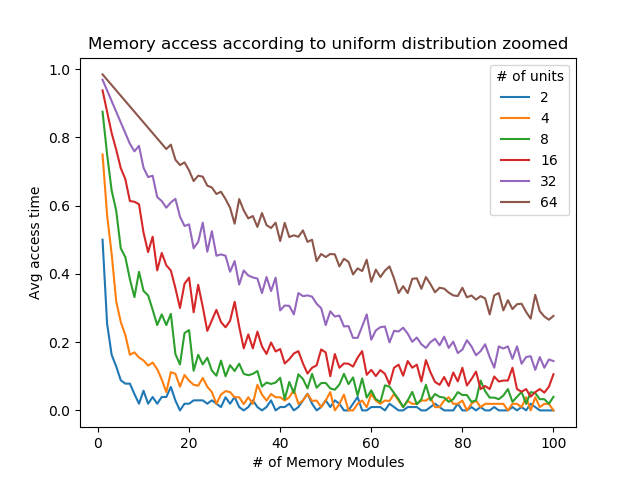
\includegraphics{uf_zoomed.png}
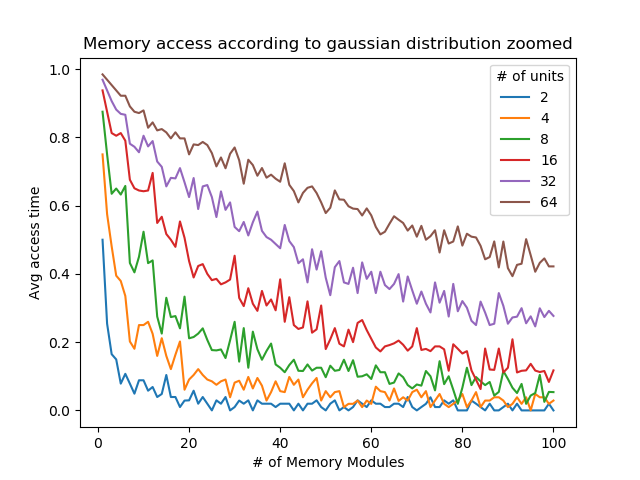
\includegraphics{gau_zoomed.png}
\centering
\end{figure}

\begin{figure}
\caption{Full range of gaussian and uniform}
\includegraphics{{uf.png}}
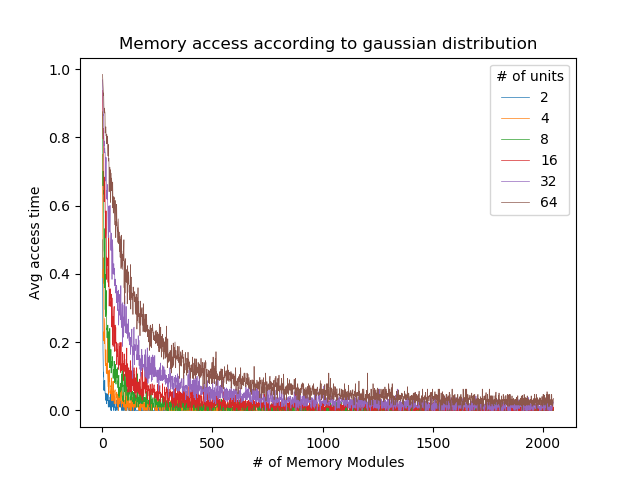
\includegraphics{gau.png}
\centering
\end{figure}

\subsection*{Observations}
\subsubsection*{More modules means faster access time}
In both graphs we see the trend that as the number of slots increase,
the average access time decreases. This is expected behavior as more slots
available decreases the probability of a collision (two units requesting the same slot). Also
as expected, when the number of units is low, the access time approaches 0 
more quickly than when the number of units is high. Take for example the blue line (units$=2$). Even when the memory of modules is only two it is unlikely that there will be a collosion.
Assuming we each unit chooses independently and uniformily at random, the probability of a collison is $\frac1{20}$!. 

\subsubsection*{Random choice according to a Uniform distribution seems to converge to 0 more quickly and with less variance than choice according to Gaussian distribution }

If you look at the two graphs, you will note that they are not perfect slopes. 
That is because in some cases we get unlucky and even though we increased the number of slots
the access time worsens then from some other simulation when we used less slots. This phenomenum is evident in both the Gaussian and Uniform plots. However, you will notice that
these so called hiccups vary in intensity. Suppose we used $a$ modules during a simulation and got access time $y_a$. Later, suppose another simulation using $a+c$ modules (where $c$
is some constant) with access time $y_{a+c}$, is such that $y_c > y_a$. The severity
of the hiccup, $H$, is how large $H = y_{a+c} - y_{a}$ is. You can see from the graphs
that all the $H$ in the guassian plot tend to be larger then the $H$ in the 
uniform plot. To see this, look at the various tick marks on the zoomed graphs, it is 
pretty much always the case that the gaussian plots have much larger hiccups at these points
then the uniform plots

\subsubsection*{A possible explanation for larger hiccups in Gaussian plots}
The problem with choosing slots according to a gaussian distribution is that all the
requests will tend to be centered around the mean. This means (not a joke) there are likely to be more collisions. This raises the question of why then does the guassian curve 
eventually approach 0 as the number of modules increases? Let's examine when $M=2048$ and 
$N=64$. In this case the standard deviation is approximately $409$ using the calculation above. Assuming in the worse case that all requests always fall within the range of $409$
of the mean, that is still a considerable amount of breathing room for the units.
Using a variation of the birtday paradox, we could determine exactly how 
likely it would be for any of the units to share the same (birthday or slot).


% import the files
\newpage
\lstinputlisting{hw1.py}
\newpage
\lstinputlisting{helper.py}
\newpage
\lstinputlisting{system.py}
\newpage

\end{document}
